\chapter{Project Planning and Organizational Development}

This chapter describes how the team organized and planned the design process during the midterm phase. The objective of the planning structure is to ensure that the remaining work is traceable, logically sequenced, and equally distributed across the team. The chapter therefore first presents the project planning tools used to decompose, connect, and schedule the work. It then describes the organizational structure used to assign responsibilities and coordinate subsystem development for the selected concept.

\section{Project Planning}
This section details the planning steps taken in order to streamline the flow of the project, while ensuring all tasks are completed. First a Work Breakdown Diagram and a Workflow Diagram were created. These were then combined to generate a Gantt Chart. All of the figures can be found on the subsequent pages.

\subsection{Work Breakdown Diagram}
The Work Breakdown Diagram (WBD) serves as the foundational framework for the project's organization. By decomposing the mission into manageable, hierarchical components, it ensures that no deliverable is overlooked and that responsibilities are clearly defined. 

\subsection{Workflow Diagram}
While the WBD defines "what" needs to be done, the Workflow Diagram (WFD) illustrates "how" the work flows through the team. It maps the technical interdependencies that dictate the project’s pace. 

Crucially, the WFD identifies "Information Bottlenecks", tasks where multiple subsystems must converge before further progress can be made, and "Parallel Tracks," where the ten-member team can work independently to maximize efficiency. Phases have to be started chronologically, while work packages can receive real-time updates in parallel with the phases. By visualizing these paths, the team can anticipate the impact of delays in one subsystem on the rest of the project, allowing for proactive resource reallocation.

This hierarchical structure allows the team to transition from high-level mission goals to specific, actionable tasks. In this project, the WBS is organized by phase, ensuring that the development follows a logical engineering lifecycle, from initial requirements capture to final validation.

\subsection{Gantt Chart}
The Gantt Chart represents the final integration of the WBS and WFD into a time-linear schedule. Generated via ENOVIA Project Planning software, this chart translates logical dependencies into specific calendar dates, accounting for the available man-hours of the team.

The primary function of the Gantt chart in this project is to monitor the Path: the sequence of tasks that directly determines the project's completion date. By tracking the resolution of tasks, down to two-hour increments, the Gantt chart provides a high-fidelity visual of project health. This level of detail is vital for ensuring that the concurrent engineering efforts remain synchronized, particularly during the transition from Preliminary to Detailed Design.

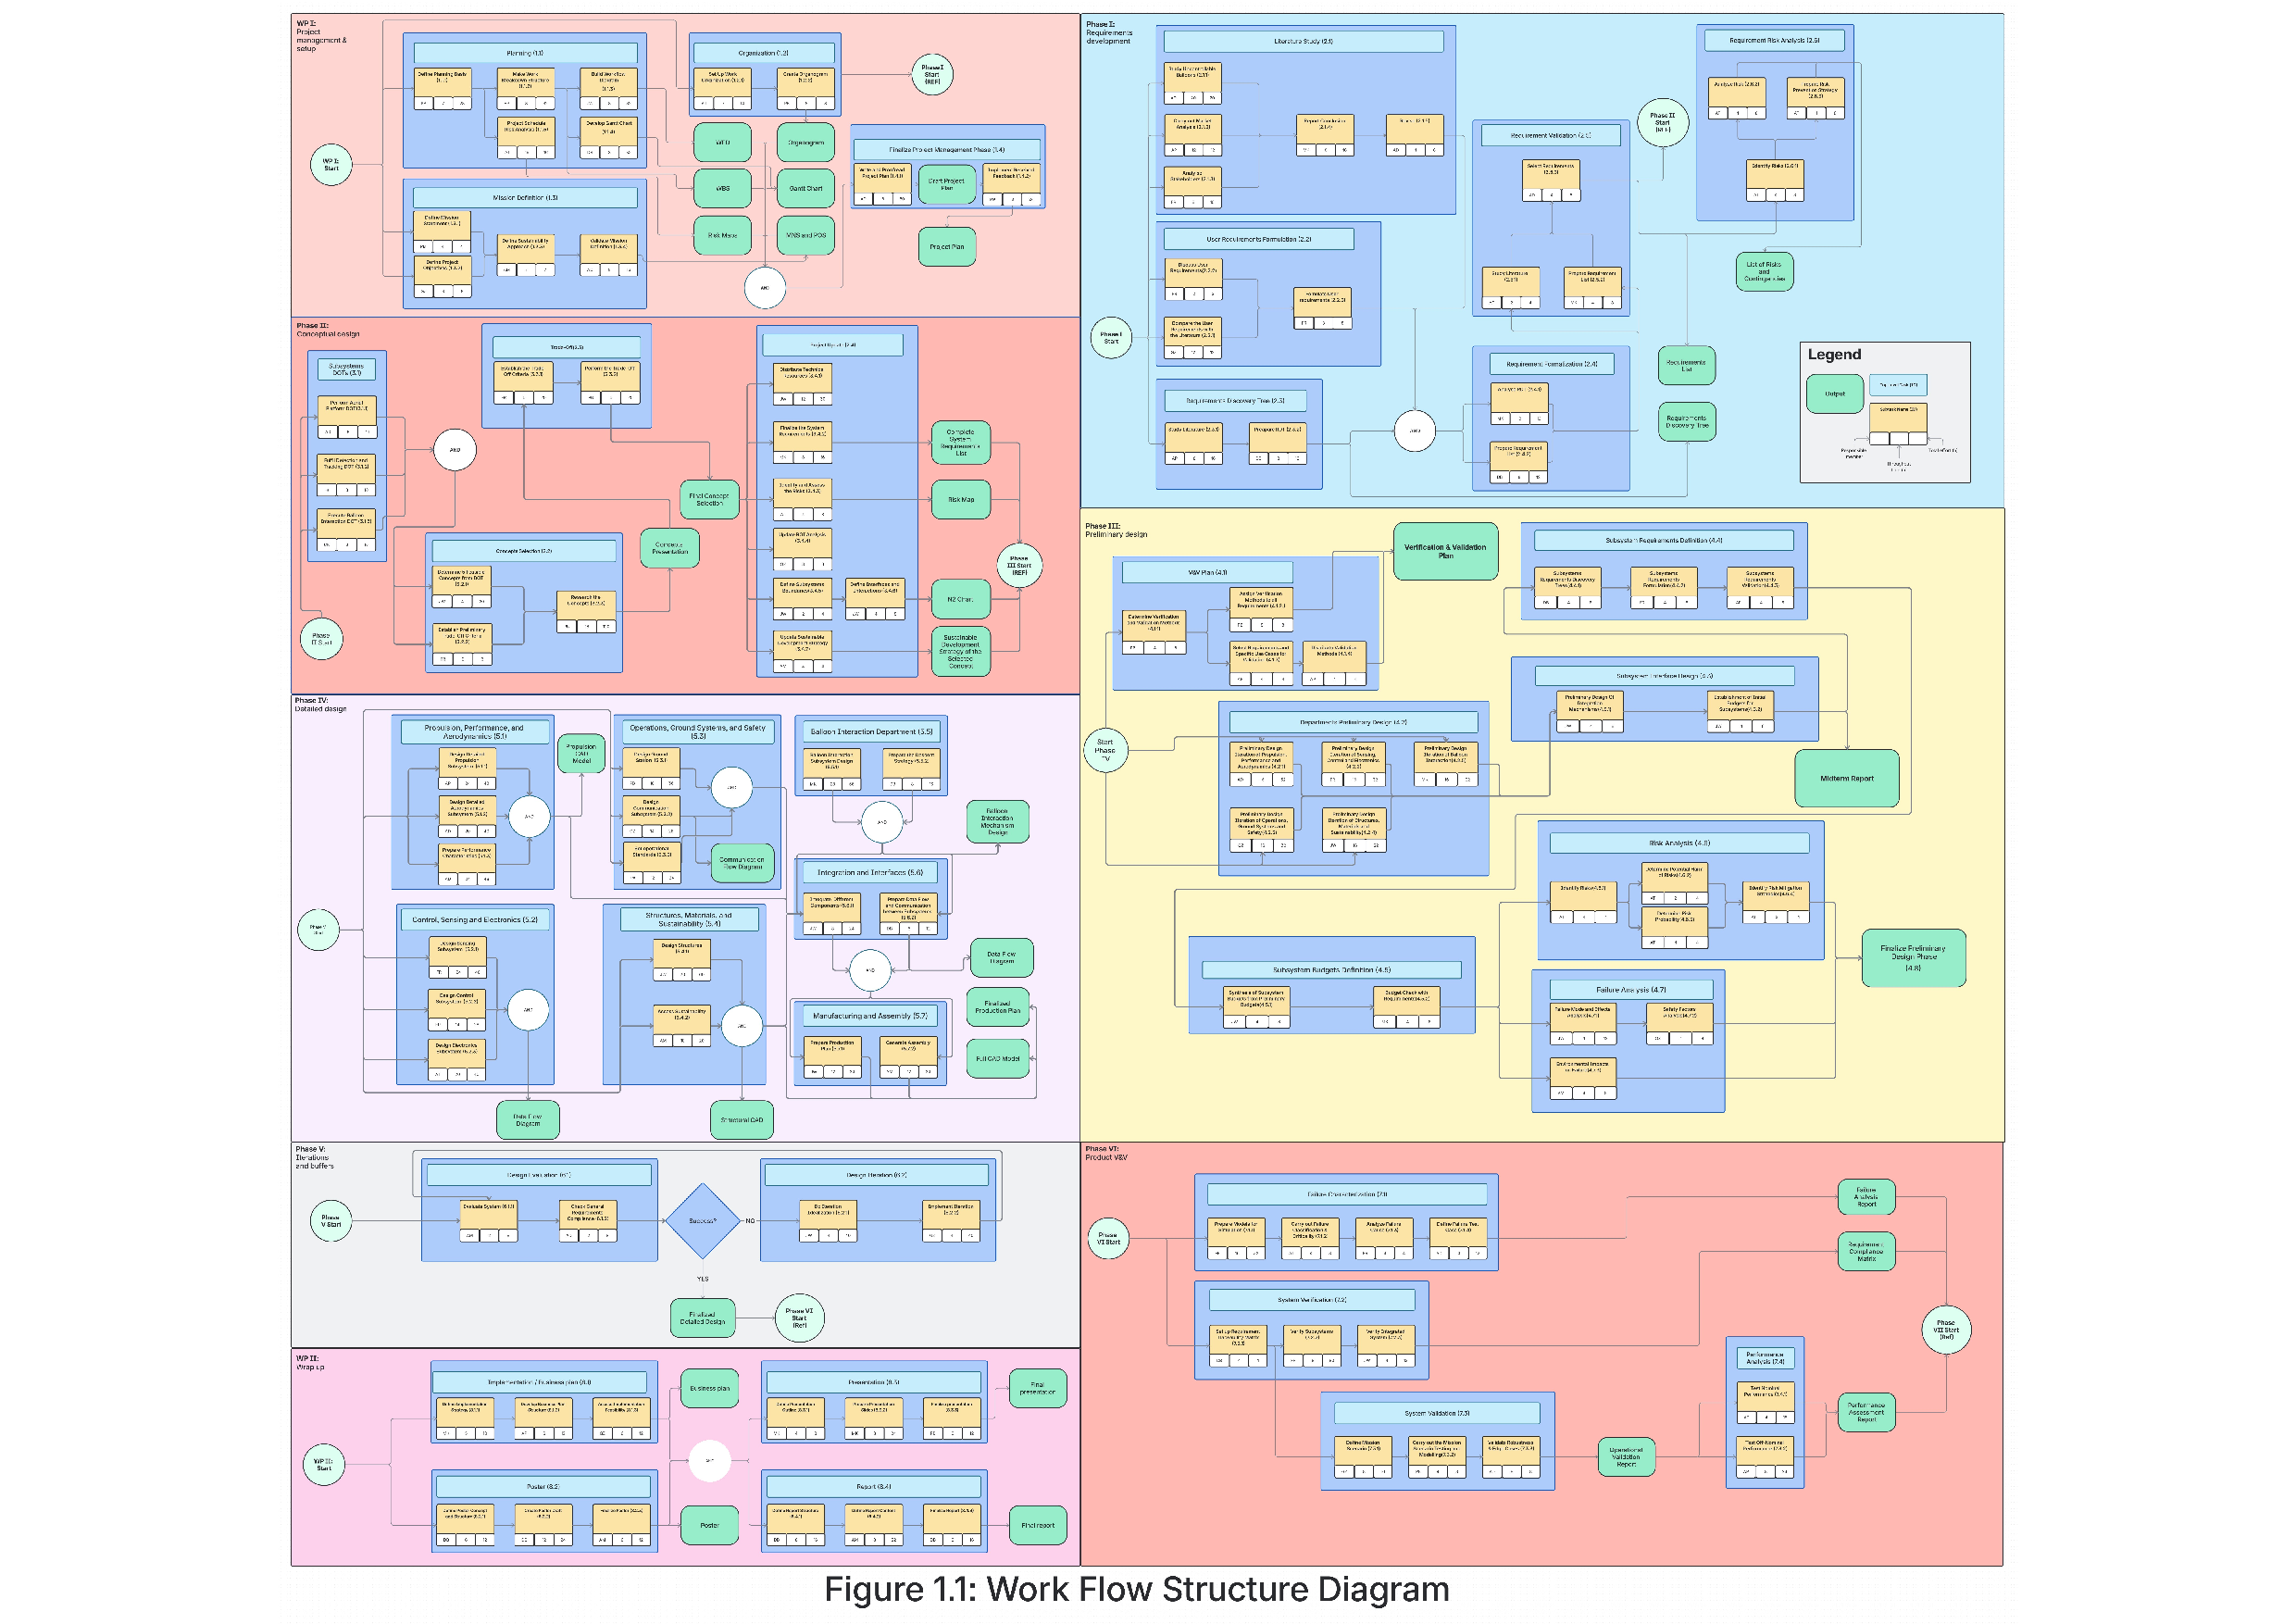
\includepdf[
     pages=-,
    fitpaper=true
]{figures/WFS_Final_Assembly.pdf}

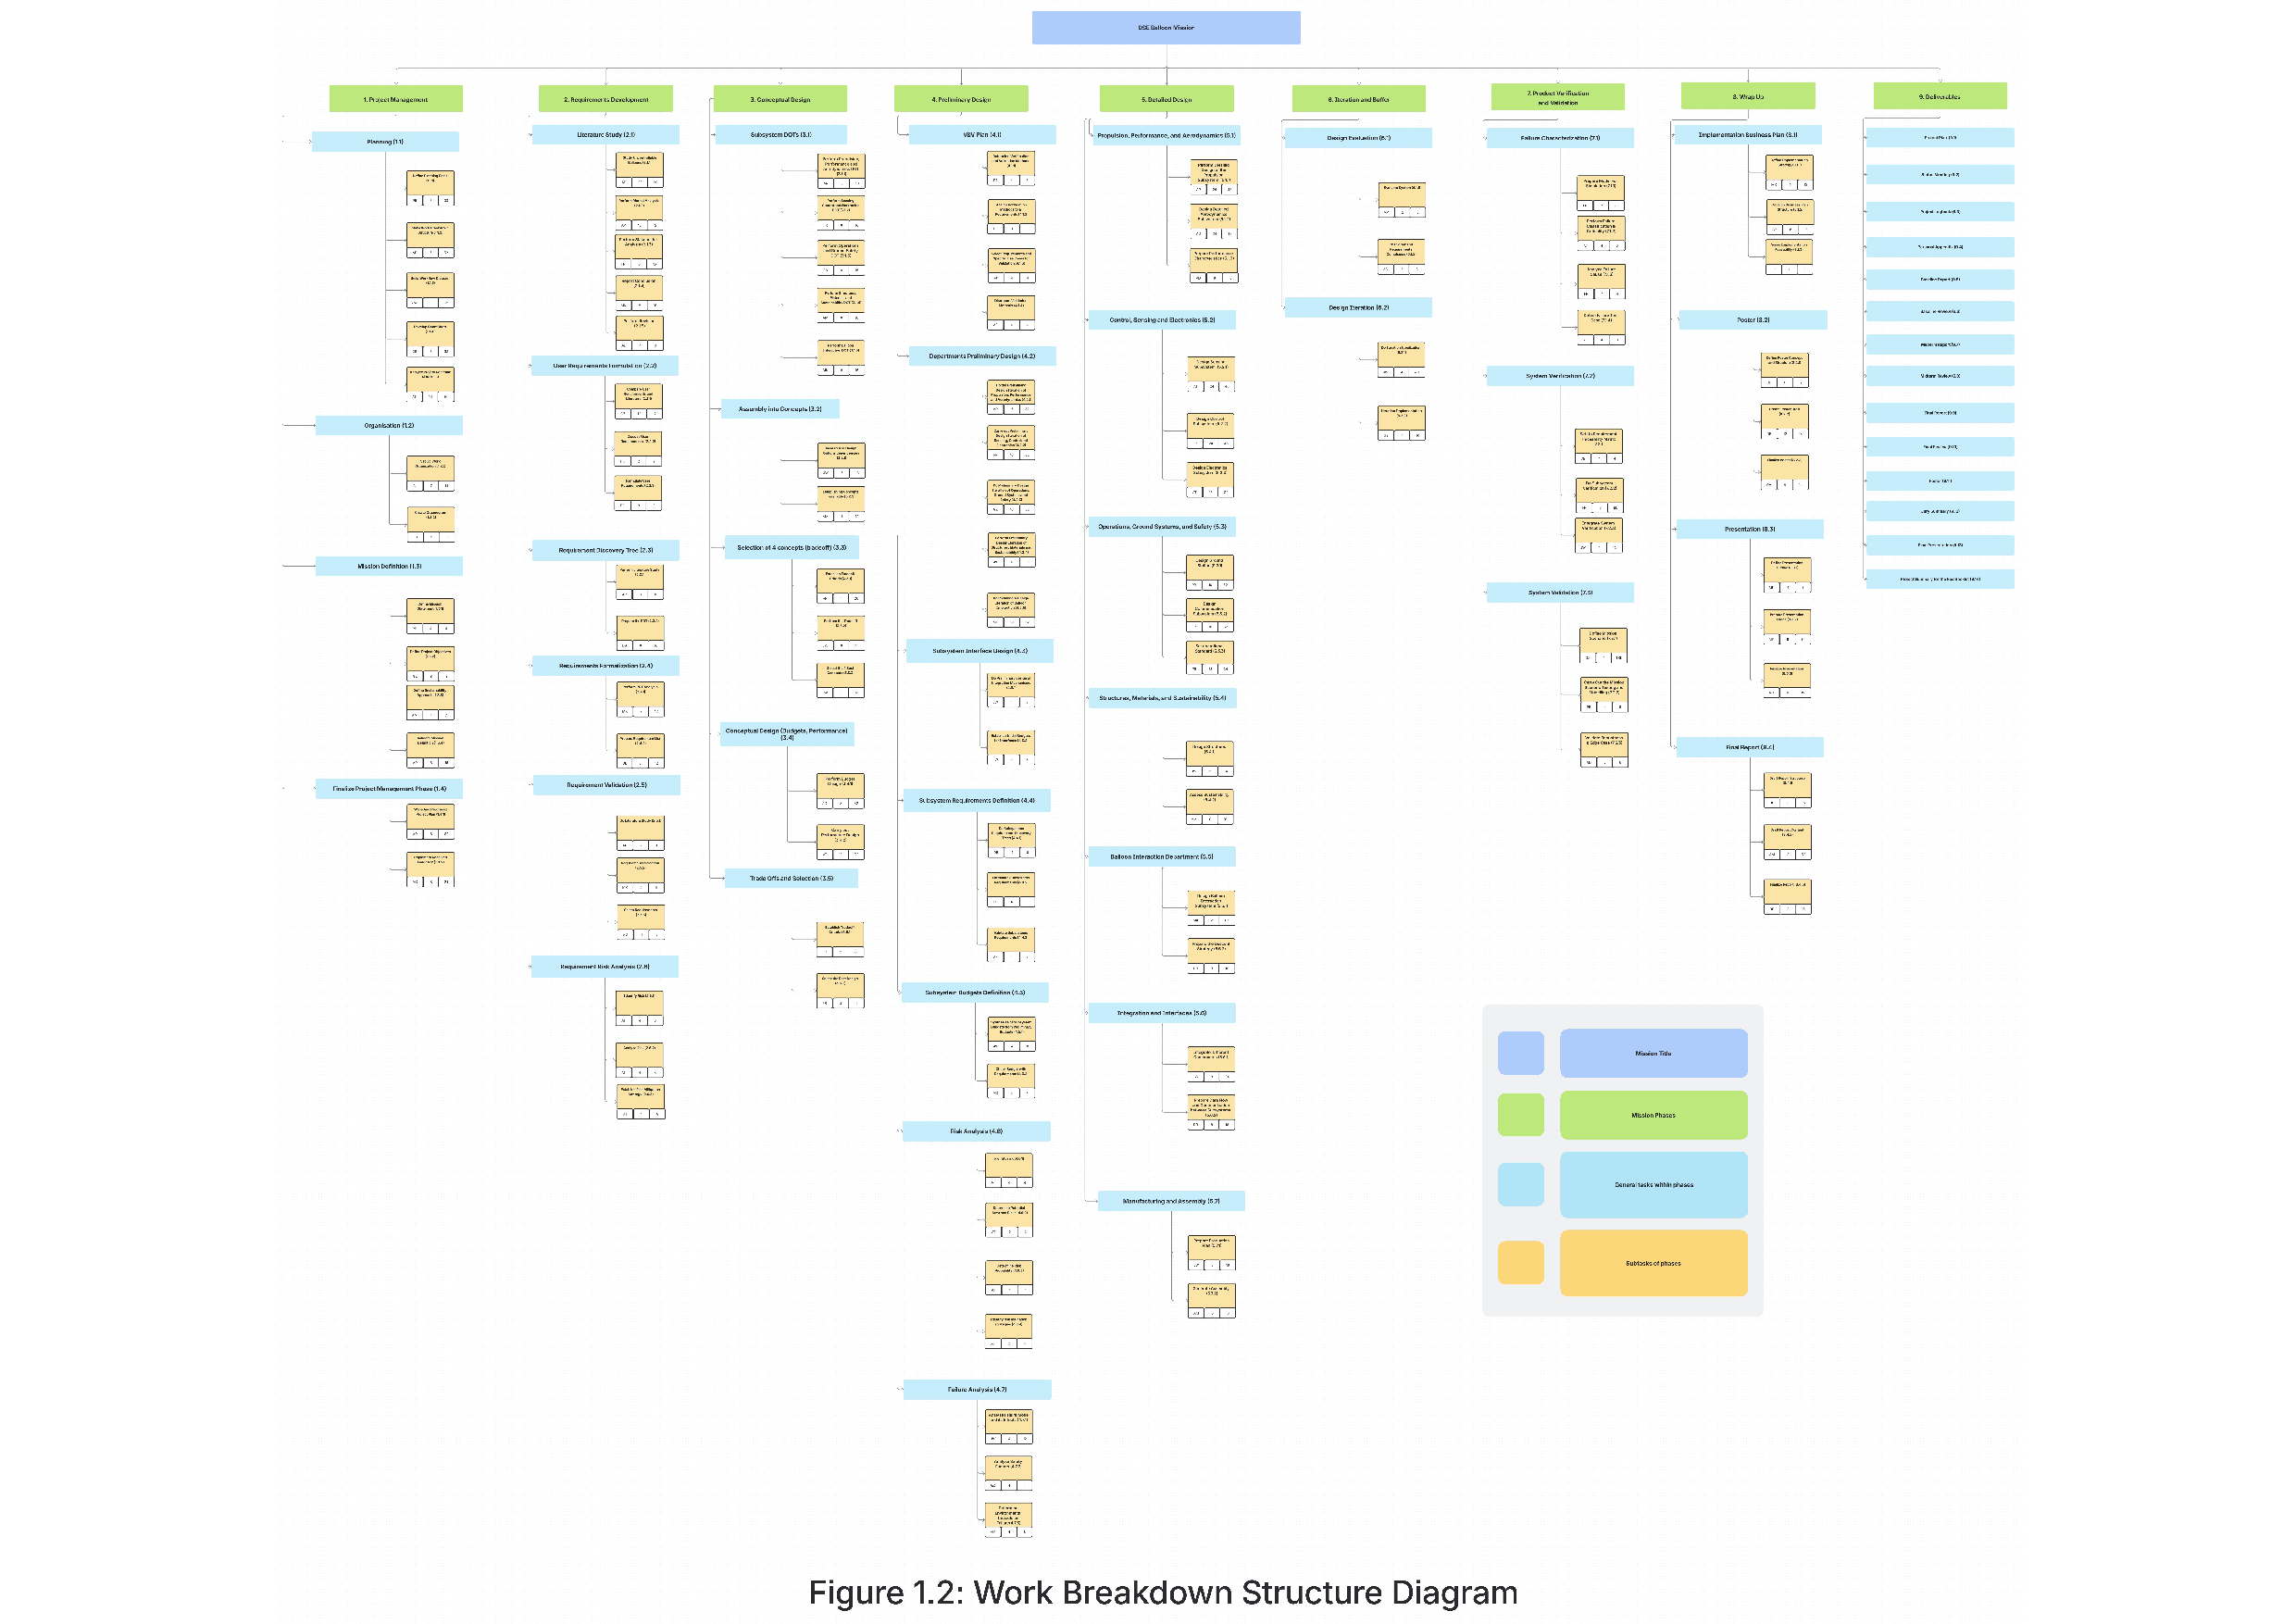
\includepdf[
     pages=-,
    fitpaper=true
]{figures/Final_WBS.pdf}



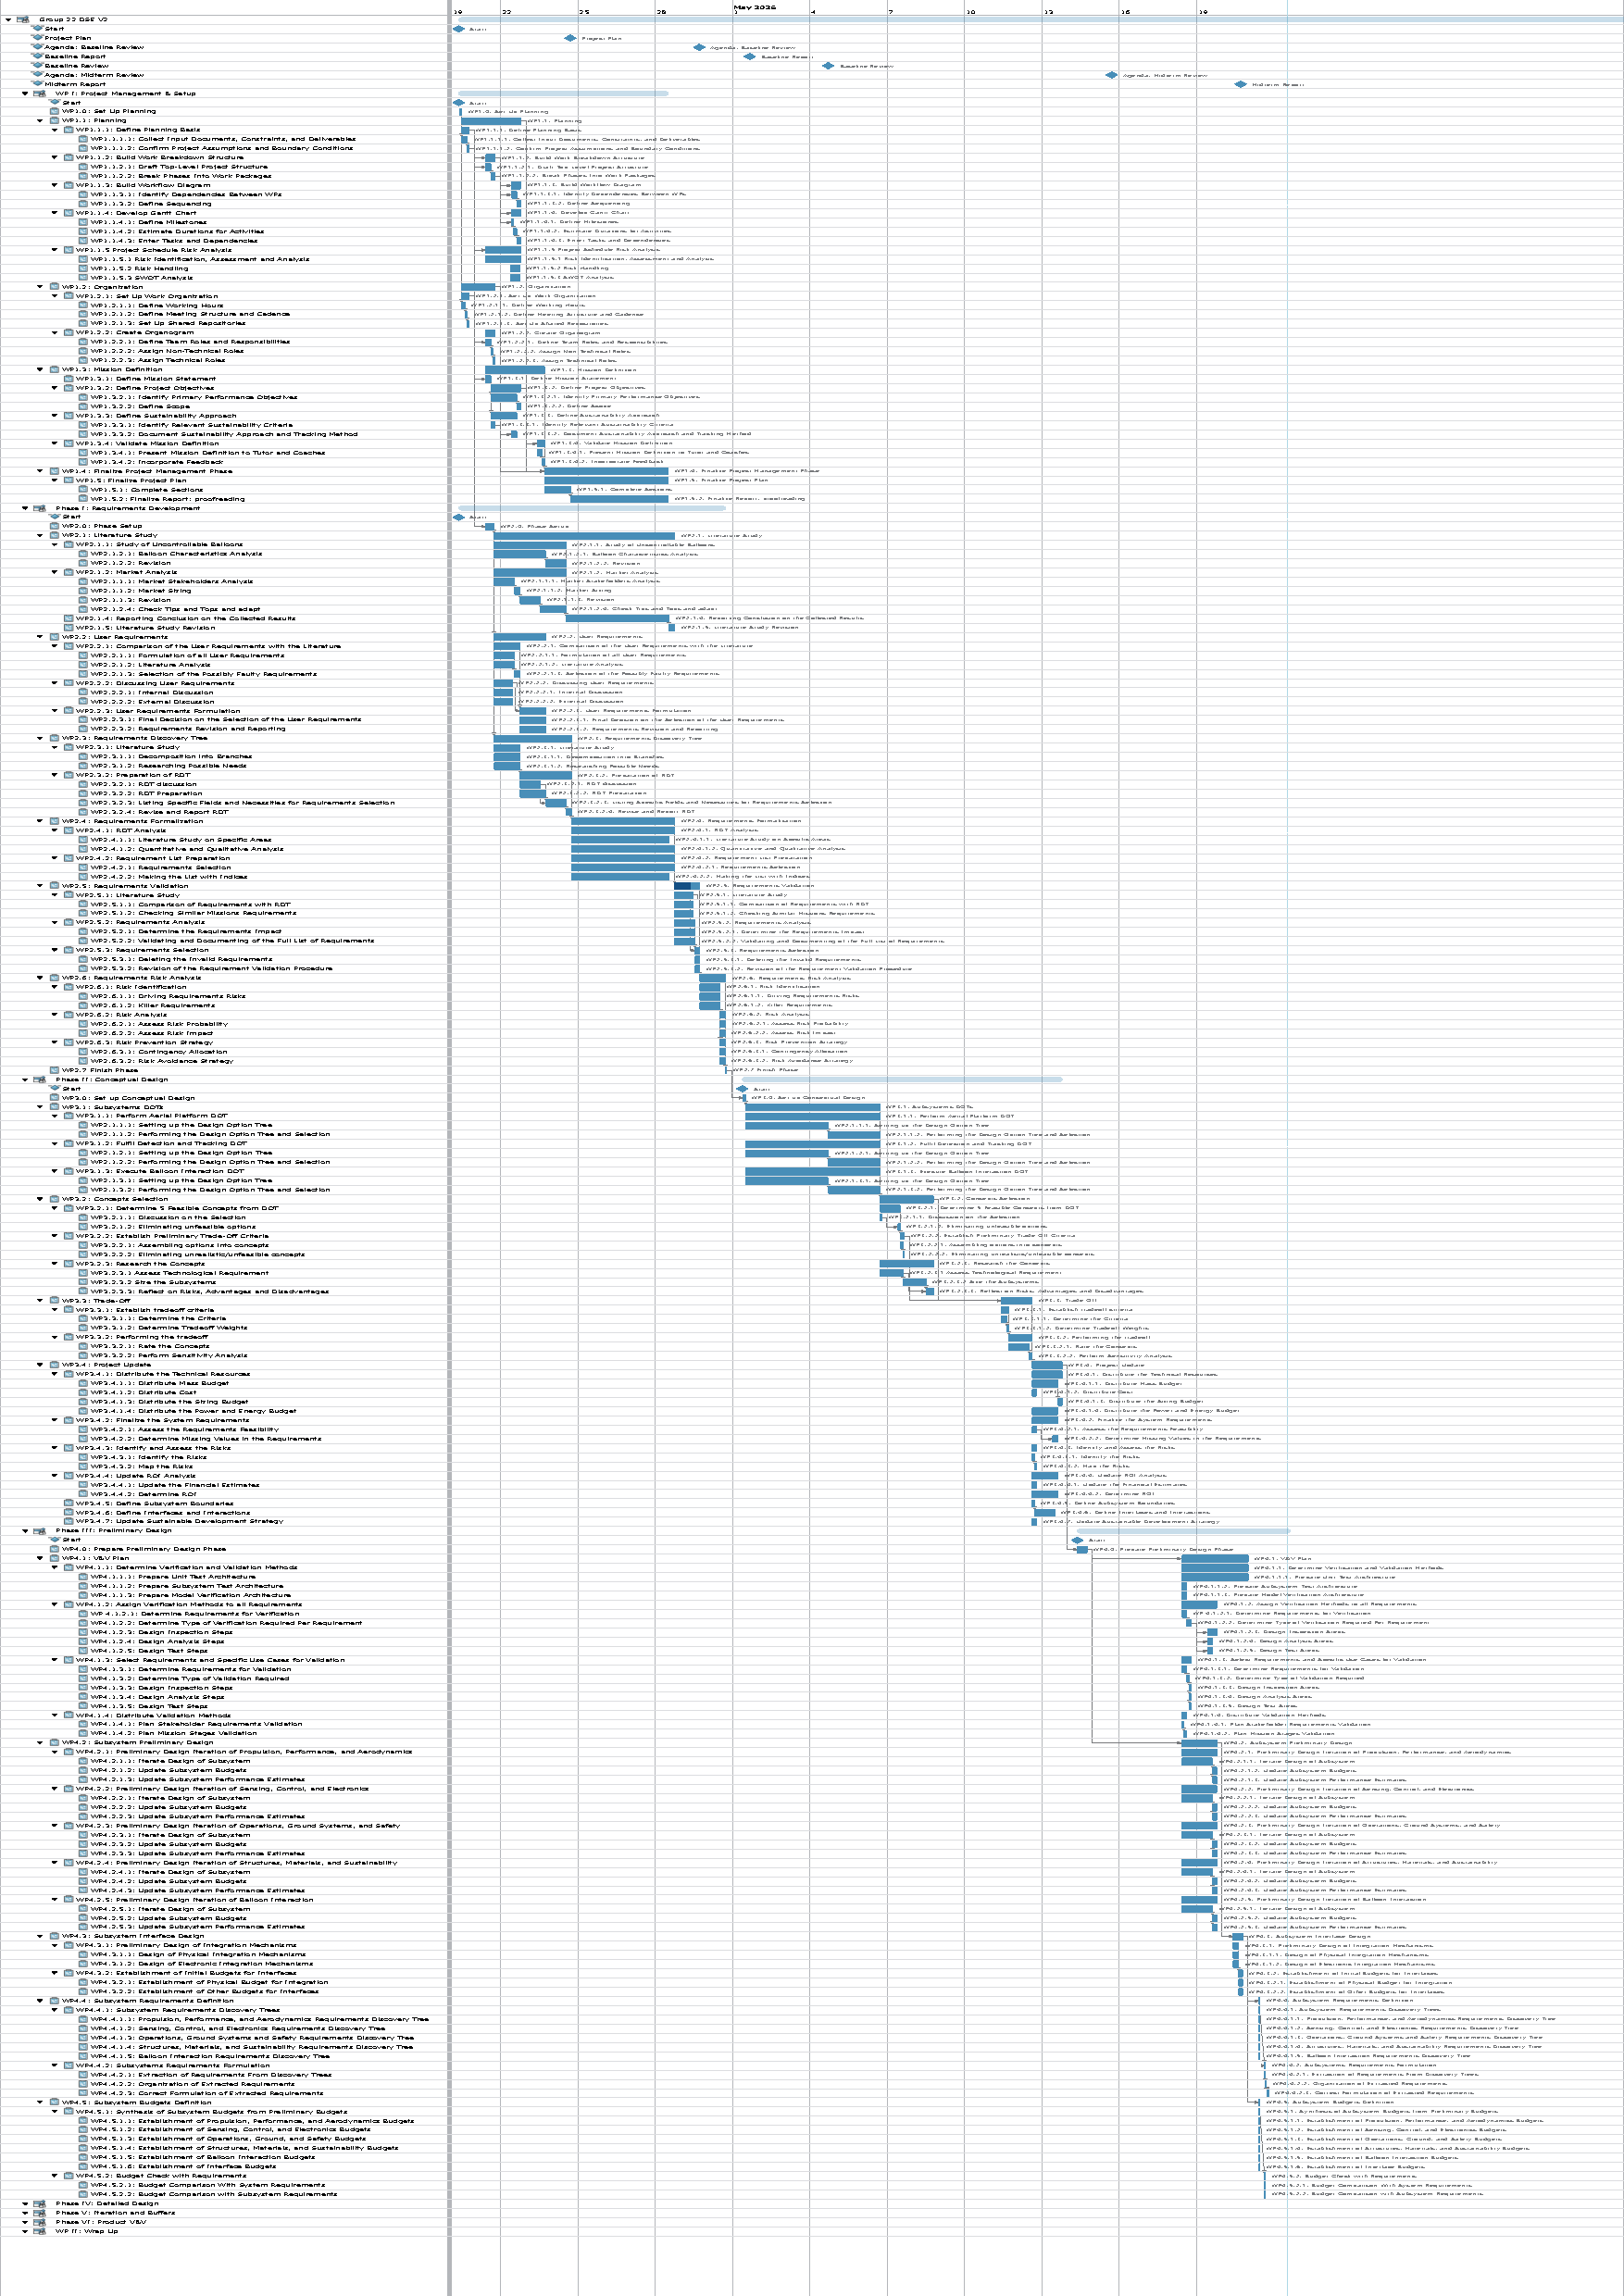
\includepdf[
    pages=-,
    landscape=true,
    fitpaper=true,
    pagecommand={\thispagestyle{plain}\vfill\captionof{figure}{Project Gantt Chart — Part 1}\label{fig:gantt_part1}}
]{figures/Group 22 DSE V2 gantt part 1 (1).pdf}

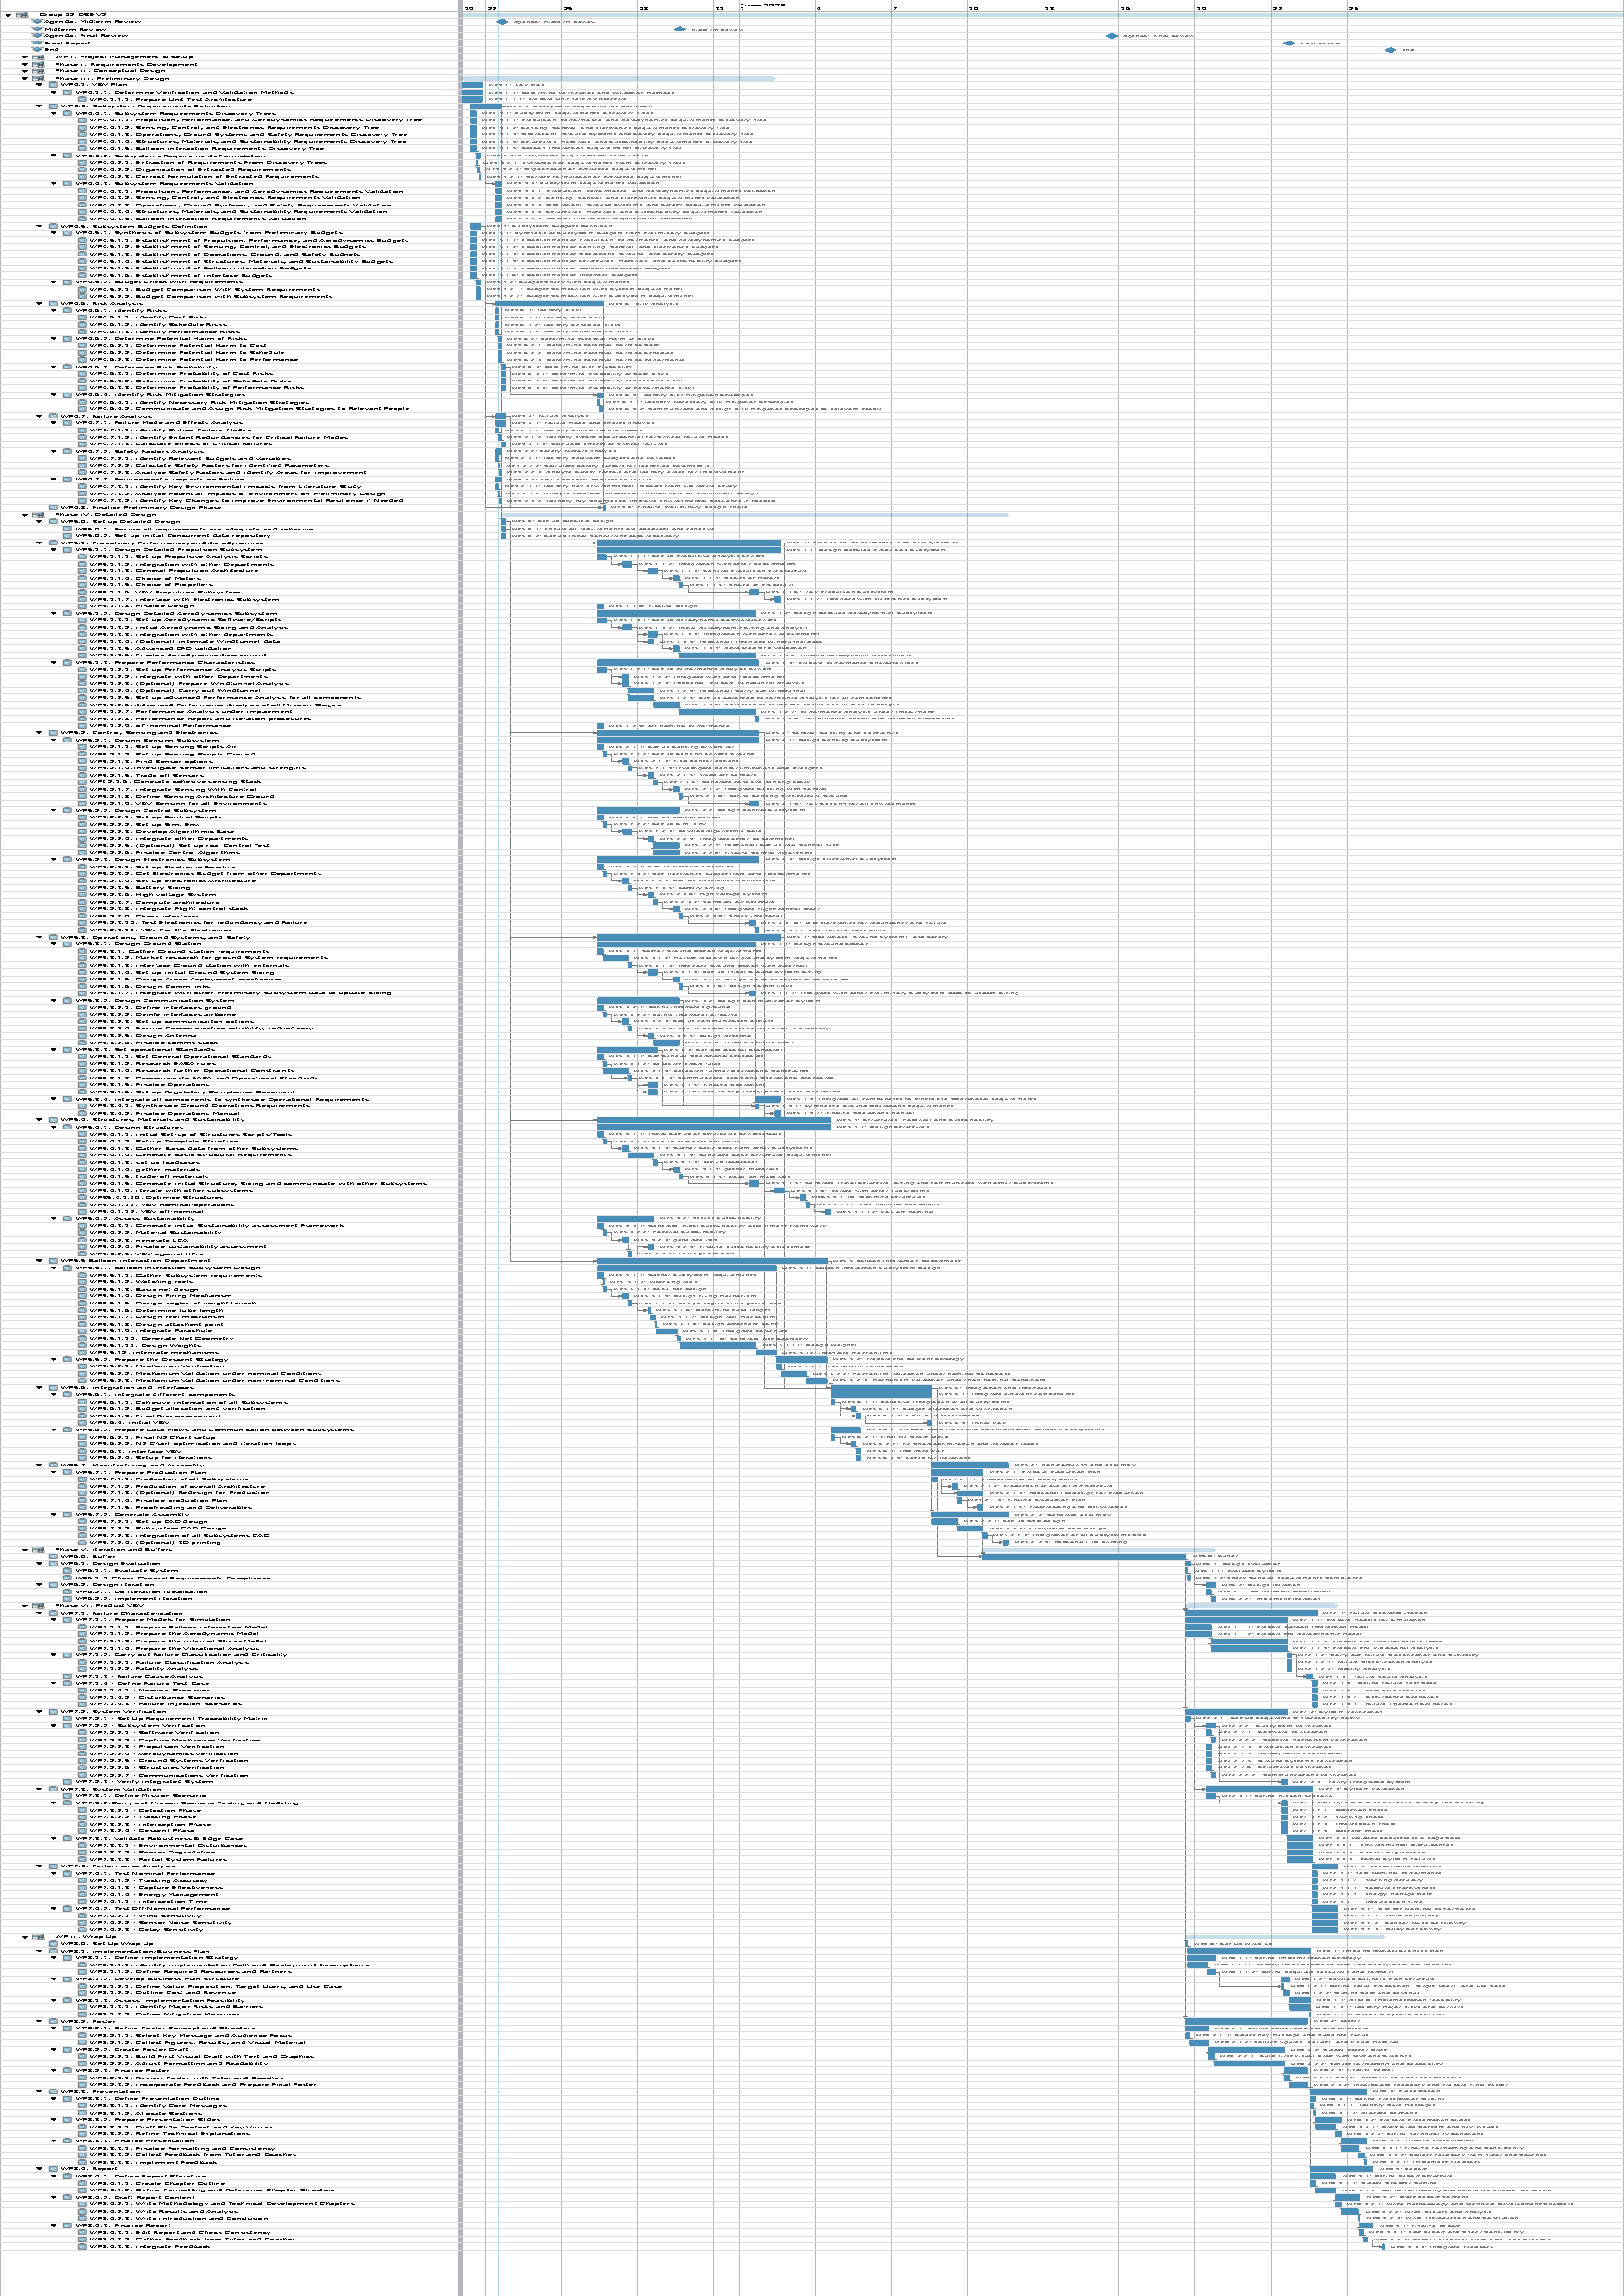
\includepdf[
    pages=-,
    landscape=true,
    fitpaper=true,
    pagecommand={\thispagestyle{plain}\vfill\captionof{figure}{Project Gantt Chart — Part 2}\label{fig:gantt_part2}}
]{figures/Group 22 DSE V2 part2 gantt (1).pdf}





\section{Organizational Development}

% \todo{roles and responsibility should be aligned with selected concepts}
To ensure good organization and clear task division, the team was split up as detailed in the Organogram: 
\begin{figure}[H]
    \centering
    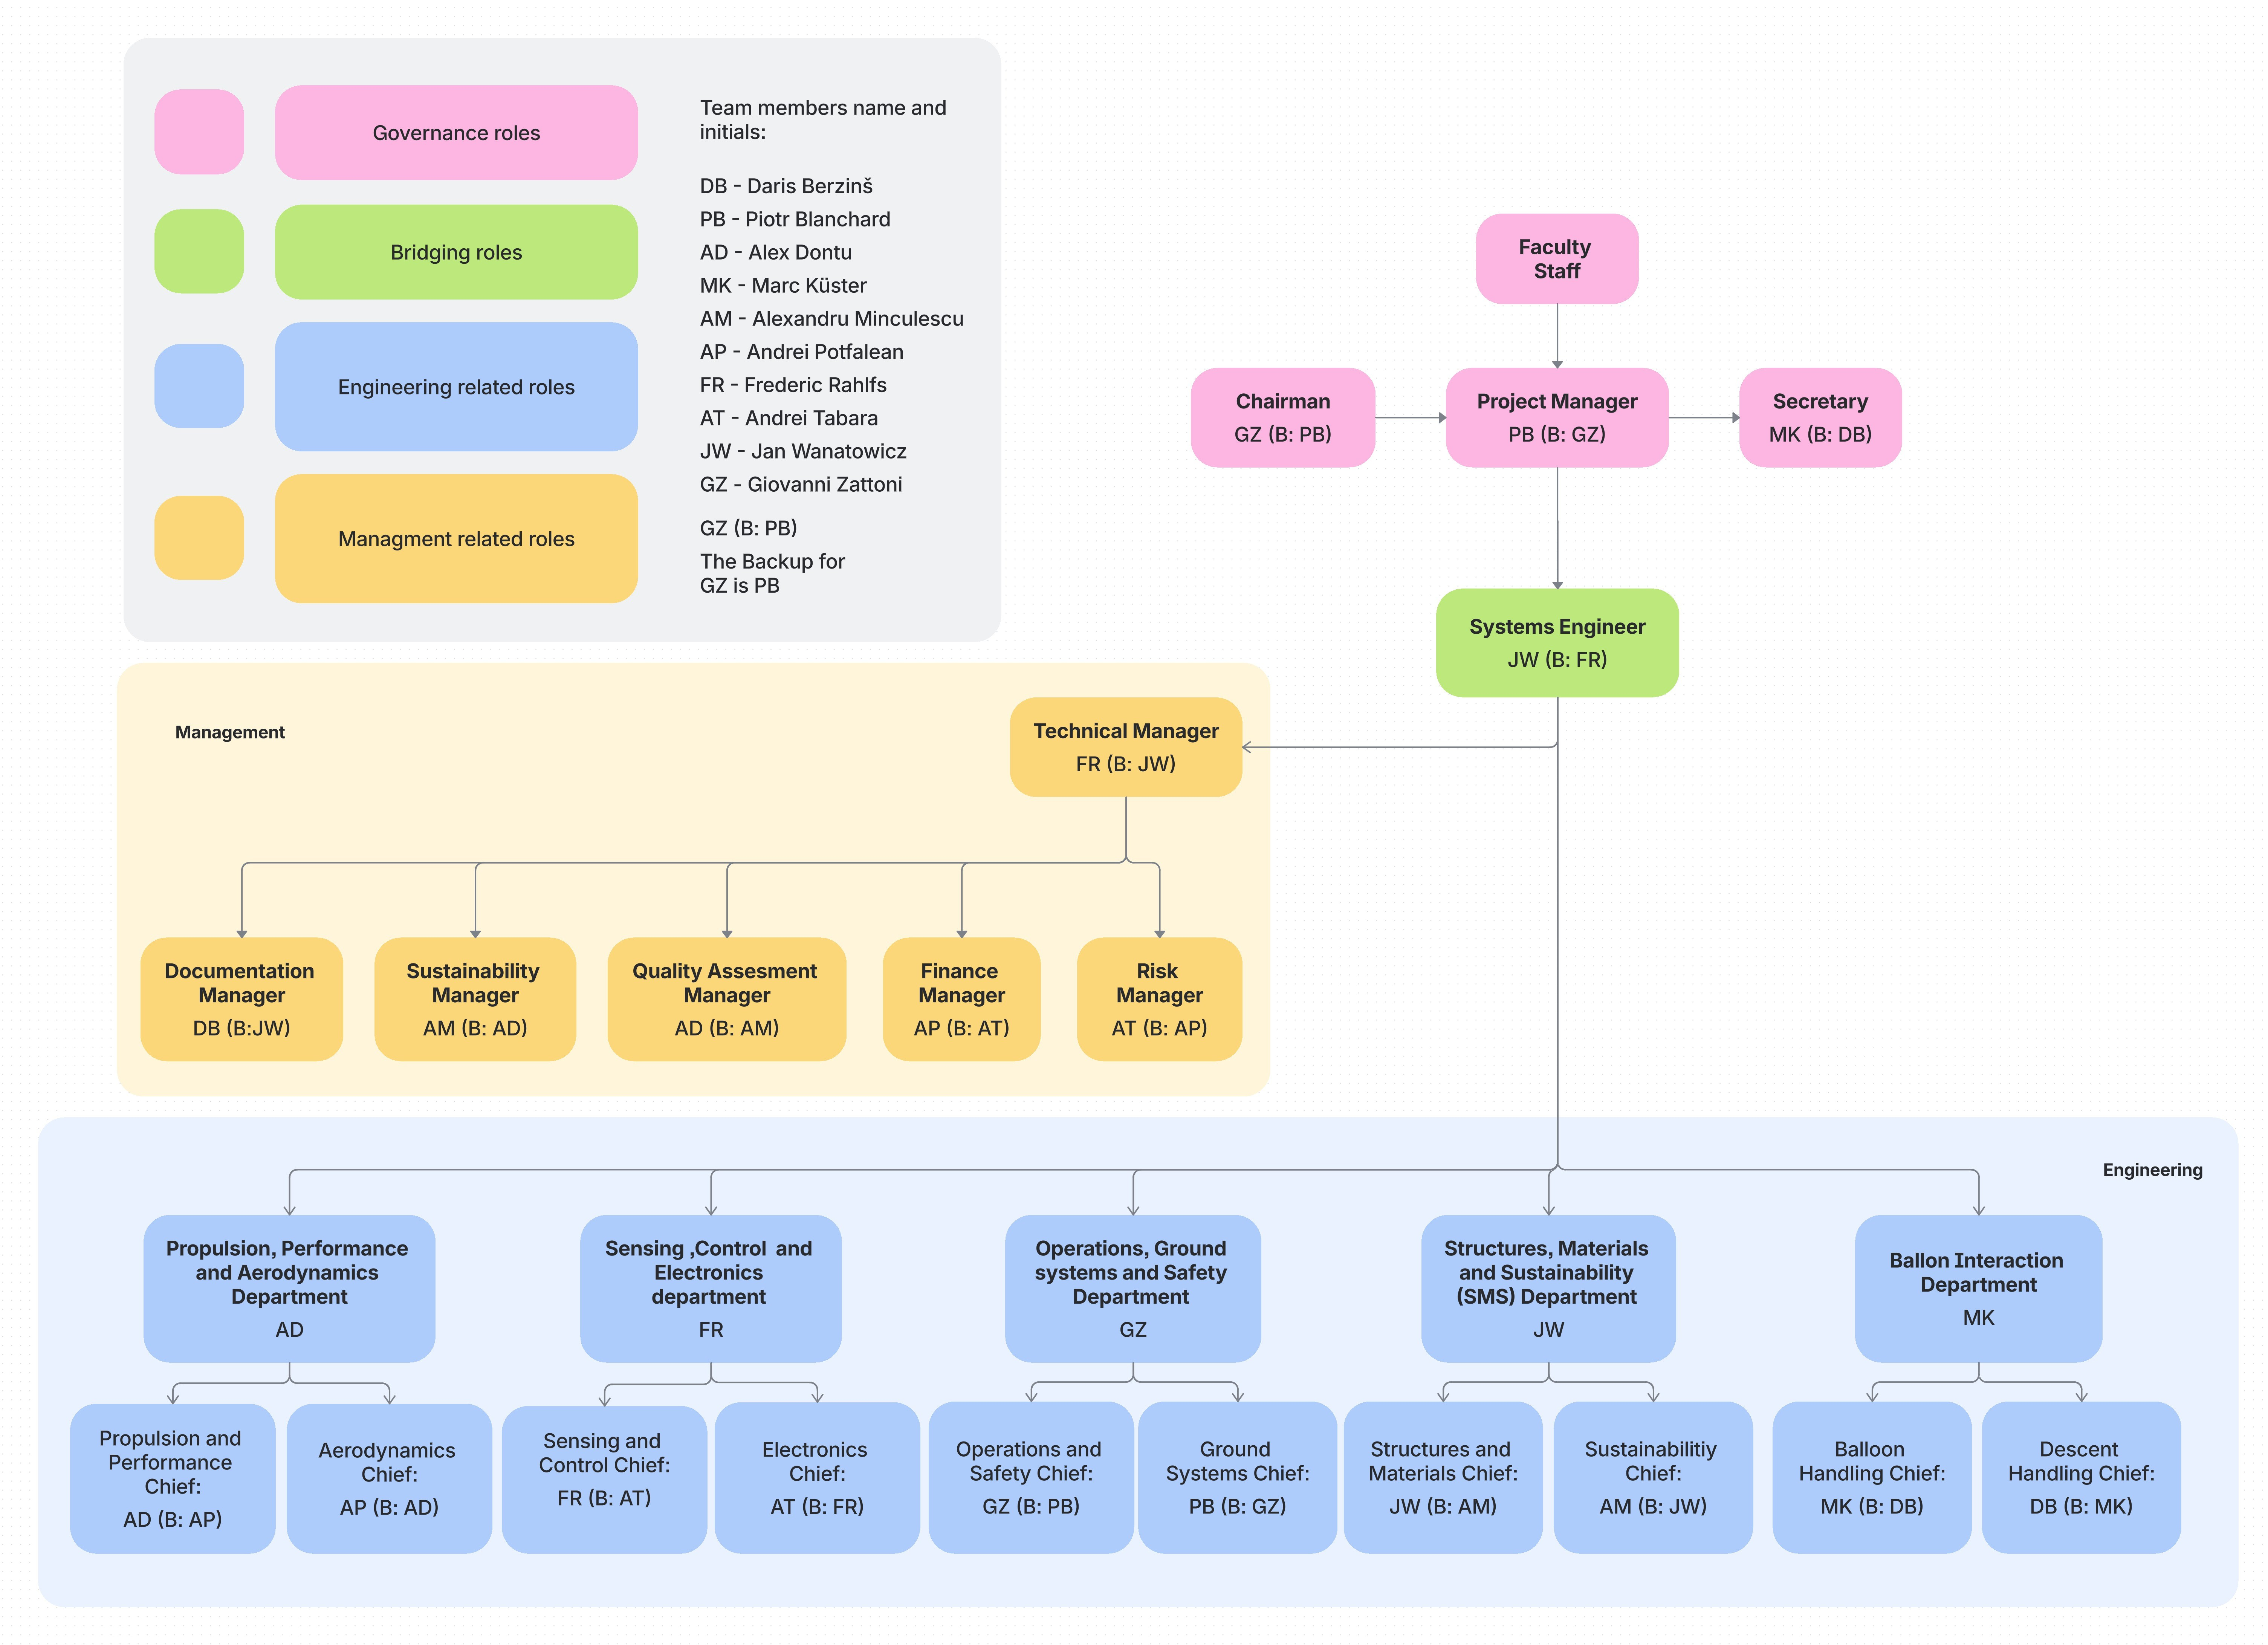
\includegraphics[width=0.8\linewidth]{figures/Organogram.jpg}
    \caption*{\textbf{Figure 1.4:} Organogram of Team Roles}
    \label{fig:organogram}
\end{figure}
This division allows subsystem owners to develop their respective design areas in parallel, while the systems engineering role maintains requirement traceability, interface consistency, and integration between subsystems.



